%\documentclass[11pt]{article}

\documentclass[a4paper,11pt]{ctexart}
\usepackage{ctex}
%
\renewcommand{\abstractname}{\zihao{4} 摘要}
\renewcommand{\contentsname}{\centering 目录}
\usepackage{fontspec}
%\setmainfont{KaiTi} % 楷体
\setmainfont{Times New Roman} % 楷体

\usepackage{gbt7714}

%自动生成文本的包 乱数假文 
%\usepackage{zhlipsum}

\usepackage{geometry}
%\geometry{a4paper,scale=0.8}
\geometry{a4paper,left=2cm,right=2cm,top=2.5cm,bottom=2.5cm}

%\usepackage{setspace}
%\setstretch{1.523}

% 给文中的链接标识
\usepackage[colorlinks,linkcolor=black,anchorcolor=blue,citecolor=green]{hyperref}

%解决图片放不下跑到文末问题
\usepackage{float}

%数学工具包
\usepackage{amsmath}
\usepackage{mathtools}
%数学单位包
\usepackage{siunitx}

%树结构图
\usepackage{forest}

%三线表
\usepackage{booktabs}
%表单元合并
\usepackage{multirow}
%图插入处理包
\usepackage{graphicx}
%指定图片存放路径img/
\graphicspath{{img/}}
%处理子图包
\usepackage{subfigure}

%处理页眉页脚
\usepackage{lastpage}
\usepackage{fancyhdr}
\pagestyle{fancy}
\fancyfoot[C]{\thepage /\pageref{LastPage}}

\chead{脸书宣布继续维持封禁特朗普账号}
\lhead{}
\rhead{}
\lfoot{来源: 人民日报 \and 新华社}

\renewcommand{\headrulewidth}{0.1mm}
\renewcommand{\footrulewidth}{0.05mm}

%图表目录
\renewcommand{\listfigurename}{\centering 图目录}
\renewcommand{\listtablename}{\centering 表目录}

\usepackage{titletoc}
\titlecontents{figure}[0.5cm]{\songti\zihao{-4}}{\figurename~\thecontentslabel\quad}{\hspace*{-1.5cm}}{\titlerule*[0.12cm]{.}\contentspage}[\addvspace{6pt}]
\titlecontents{table}[0.5cm]{\songti\zihao{-4}}{\tablename~\thecontentslabel\quad}{\hspace*{-1.5cm}}{\titlerule*[0.12cm]{.}\contentspage}[\addvspace{6pt}]
%\bf加粗 设置目录标题
\titlecontents{section}[0.5cm]{\songti\zihao{-4}}{\bfseries\thecontentslabel\quad}{\hspace*{-1.5cm}}{\titlerule*[0.12cm]{.}\contentspage}[\addvspace{6pt}]
\titlecontents{subsection}[1.5cm]{\songti\zihao{5}}{\thecontentslabel\quad}{\hspace*{-1.5cm}}{\titlerule*[0.12cm]{.}\contentspage}[\addvspace{6pt}]
%
\titlecontents{chapter}[2.7cm]{\songti\zihao{-4}}{\bf\thecontentslabel\quad}{\hspace*{-1.5cm}}{\titlerule*[0.12cm]{.}\contentspage}[\addvspace{6pt}]

\usepackage{titlesec}

\title{\heiti 脸书宣布继续维持封禁特朗普账号}
\author{张三\thanks{单位:人民日报;邮箱:xxx@mail.cn} \and 李四\thanks{Corresponding author} \and 王五}
\date{\today}


\begin{document}
	\maketitle
	
	\begin{abstract}
		\large
		{\kaishu 当地时间5月5日,美国社交媒体平台脸书(Facebook)的独立监督委员会投票决定,美国前总统特朗普(图\ref{特兰普2})的相关账号将继续维持“无限期”被封禁状态,并要求脸书在六个月内重新发布审查结果以及决定惩罚措施。}
	\end{abstract}
	%设置间距
	\vspace{1cm}
	% 生成目录
	\tableofcontents
%	
%	%生成图表目录
	\listoffigures
	\listoftables
	
	%换页
	\newpage
	
	\section{限制特朗普访问脸书}
	{\kaishu 独立监督委员会表示“维持了脸书在2021年1月7日的决定,即限制时任总统特朗普(图\ref{特兰普3})访问其脸书和Instagram页面发布内容。”但同时表示,“脸书不宜无限期执行这种封禁。脸书的普通惩罚包括移除违反规定的内容、执行一段时间封号或彻底进行封禁。(图 \ref{t1})”}
	% H为float包参数 解决图片过大排版跑到文末的问题
	\begin{figure}[H]
		\centering
		\subfigure[特朗普1]{
			\centering
			
\includegraphics[scale=0.5]{tlp}
			\label{特兰普1}
			}
		\subfigure[特兰普2]{
			\centering
			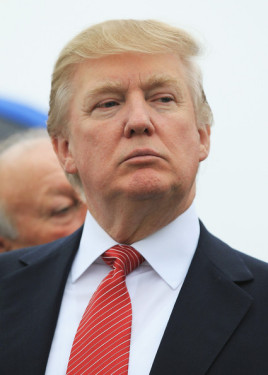
\includegraphics[scale=0.5]{tlp2}
			\label{特兰普2}}
		\subfigure[特兰普3]{
			\centering
			
\includegraphics[scale=0.5]{tlp}
			\label{特兰普3}
			}
		\caption{特朗普2016-2020}
		\label{特朗普2016-2020}
	\end{figure}
	\subsection{重返白宫坚实一步}
	据美国媒体报道,美国前总统特朗普推出了自己的交流平台,该平台名为“来自唐纳德·J·特朗普的办公桌”,特朗普可以在平台上发帖、上传照片和视频。该平台的主要作用不是交流,由于只有特朗普自己能够在上面发声,所以只能实现单向交流,不过这对于特朗普来说已经够用了,特朗普不在乎其他人说什么,只要自己发表内容有人能看到就行。
	
	行内公式:$ n = 5$
	\begin{equation}
		\begin{aligned}
			& a^2 + b^2 = c^2
		\end{aligned}
	\end{equation}
	\begin{equation}
		\begin{aligned}
			& \num{-1.236e96} \\
			& \SI{28984455224}{m/s}
		\end{aligned}
	\end{equation}
	\subsection{重返白宫胜利在望}
	此外,该平台还有一个非常鸡贼的地方,可以将这个平台上的内容分享到其他其他平台。以后特朗普只要在自己的平台上发号施令就行,支持者们自然会将他的言论分享到其他的平台上。如此一来,美国多家社交媒体对特朗普的封锁也就形同虚设了。
	之前,一直有声音称,特朗普将打造自己的社交媒体平台,现在说到做到,拿出了成品。虽然跟成熟的社交媒体平台没法比,但是对于特朗普来说,已经够用了。关键的地方在于,特朗普在自己的平台上可以为所欲为,没有人能够阻挡他乱说话。
	之前,社交媒体平台集体针对特朗普,在疫情暴发之后,特朗普的很多言论都被平台给“夹了”,最终甚至直接被永久封锁。现在好了,没有人能折叠特朗普的言论,也没有人能封锁他发声的渠道,对于重返白宫来说,迈出了坚实的一步。
	特朗普本就是一个社交媒体达人,在社交媒体上,特朗普不只是娱乐、玩票,在一定程度上,确实可以看成是“治国工具”。尤其是在煽动国会骚乱的时候,社交媒体发挥了巨大的作用,给他的支持者们,指明了道路。
	近日,特朗普已经给出了明确的回应,证实自己将会参加2024年的大选,对于他的年龄来说,这是特朗普重返白宫最后的机会了。在美国历史上,仅出现过一次类似的情况,格罗弗·克利夫兰就曾分开担任了两届美国总统,他在1885年到1889年第一次担任总统,竞选连任的时候失利,然后去当了几年律师,于1893年再次竞选,成功重返白宫。
	\begin{figure}
		\centering
		\begin{forest}
			[A [B [D] [E]] [C [X] [Y]]]]
		\end{forest}
		\caption{流程图}
	\end{figure}
	
	\section{特朗普账户仍将继续暂停}
	在一份声明中,脸书回应委员会称,将考虑董事会决定,但特朗普账户仍将继续暂停。民权专家表示,这起案件中特朗普是否被封禁的决定将对社交媒体平台上的内容审核产生巨大影响\cite{adams1995hitchhiker,王征2017基于卷积神经网络和}。
	\begin{figure}[H]
		\centering
		
\includegraphics[scale=0.5]{tlp}
		\caption{特兰普2016}
		\label{fig:tlp2016}
	\end{figure}
	
	此前脸书在1月6日美国国会暴力事件后,暂时“无限期”封禁了特朗普的账户,后来监督委员会听取了来自特朗普方的上诉并审核其账号发表内容是否敏感、引发争议及煽动暴力。
	\begin{figure}[H]
		\centering
		\subfigure[特朗普1]{
\includegraphics[width=4.5cm]{tlp}\label{t1}}
		\quad
		\subfigure[特朗普2]{
\includegraphics[width=4.5cm]{tlp}\label{t2}}
		\quad
		
		\subfigure[特朗普3]{
\includegraphics[width=4.5cm]{tlp}\label{t3}}
		\quad
		\subfigure[特朗普4]{
\includegraphics[width=4.5cm]{tlp}\label{t4}}
		\caption{特朗普}
	\end{figure}

	\section{特朗普简介}
	特朗普于1968年获得宾夕法尼亚大学沃顿商学院经济学学士学位,随后任职于父亲弗雷德·特朗普的房地产公司。1971年接管公司,从事房地产开发,投资范围逐步延伸至其他多个行业(表\ref{tab:addlabel1})。特朗普于2015年6月以美国共和党人身份宣布参选美国总统,2016年11月9日当选美国第45任总统,2017年1月20日宣誓就职。2020年12月,特朗普败选,连任失败(表 \ref{tab:addlabel2})。2021年1月19日,特朗普发表告别演说。
	% Table generated by Excel2LaTeX from sheet 'Sheet1'
	\begin{table}[H]
		\centering
		\caption{Add caption}
		\begin{tabular}{cccc}
			\toprule
			& Grow Speed & User Quanlity & Is Sign \\
			\midrule
			2016  & 6.80\% & 18823 & Y \\
			2017  & 6.90\% & 185247 & F \\
			2018  & 6.80\% & 58972 & F \\
			2019  & 8.90\% & 225584 & Y \\
			2020  & 2.10\% & 222544 & F \\
			2021  & 5.80\% & 6687452 & Y \\
			2022  & 6.70\% & 55799522 & F \\
			\bottomrule
		\end{tabular}%
		\label{tab:addlabel1}%
	\end{table}%
	
%	 Table generated by Excel2LaTeX from sheet 'Sheet1'
	\begin{table}[H]
		\centering
		\caption{Add caption}
		\begin{tabular}{ccccc}
			\toprule
			& Grow Speed & User Quanlity & Is Sign & Level \\
			\midrule
			2016  & 6.80\% & 18823 & Y     & \multirow{3}[1]{*}{L} \\
			2017  & 6.90\% & 185247 & F     &  \\
			2018  & 6.80\% & 58972 & F     &  \\
			2019  & 8.90\% & 225584 & Y     & \multirow{4}[1]{*}{H} \\
			2020  & 2.10\% & 222544 & F     &  \\
			2021  & 5.80\% & 6687452 & Y     &  \\
			2022  & 6.70\% & 55799522 & F     &  \\
			\bottomrule
		\end{tabular}%
		\label{tab:addlabel2}%
	\end{table}%
	
	\clearpage
	\phantomsection
	\addcontentsline{toc}{chapter}{\centering 参考文献}
	\bibliography{zhref}

\end{document}